\begin{knitrout}
\definecolor{shadecolor}{rgb}{0.969, 0.969, 0.969}\color{fgcolor}\begin{figure}

{\centering 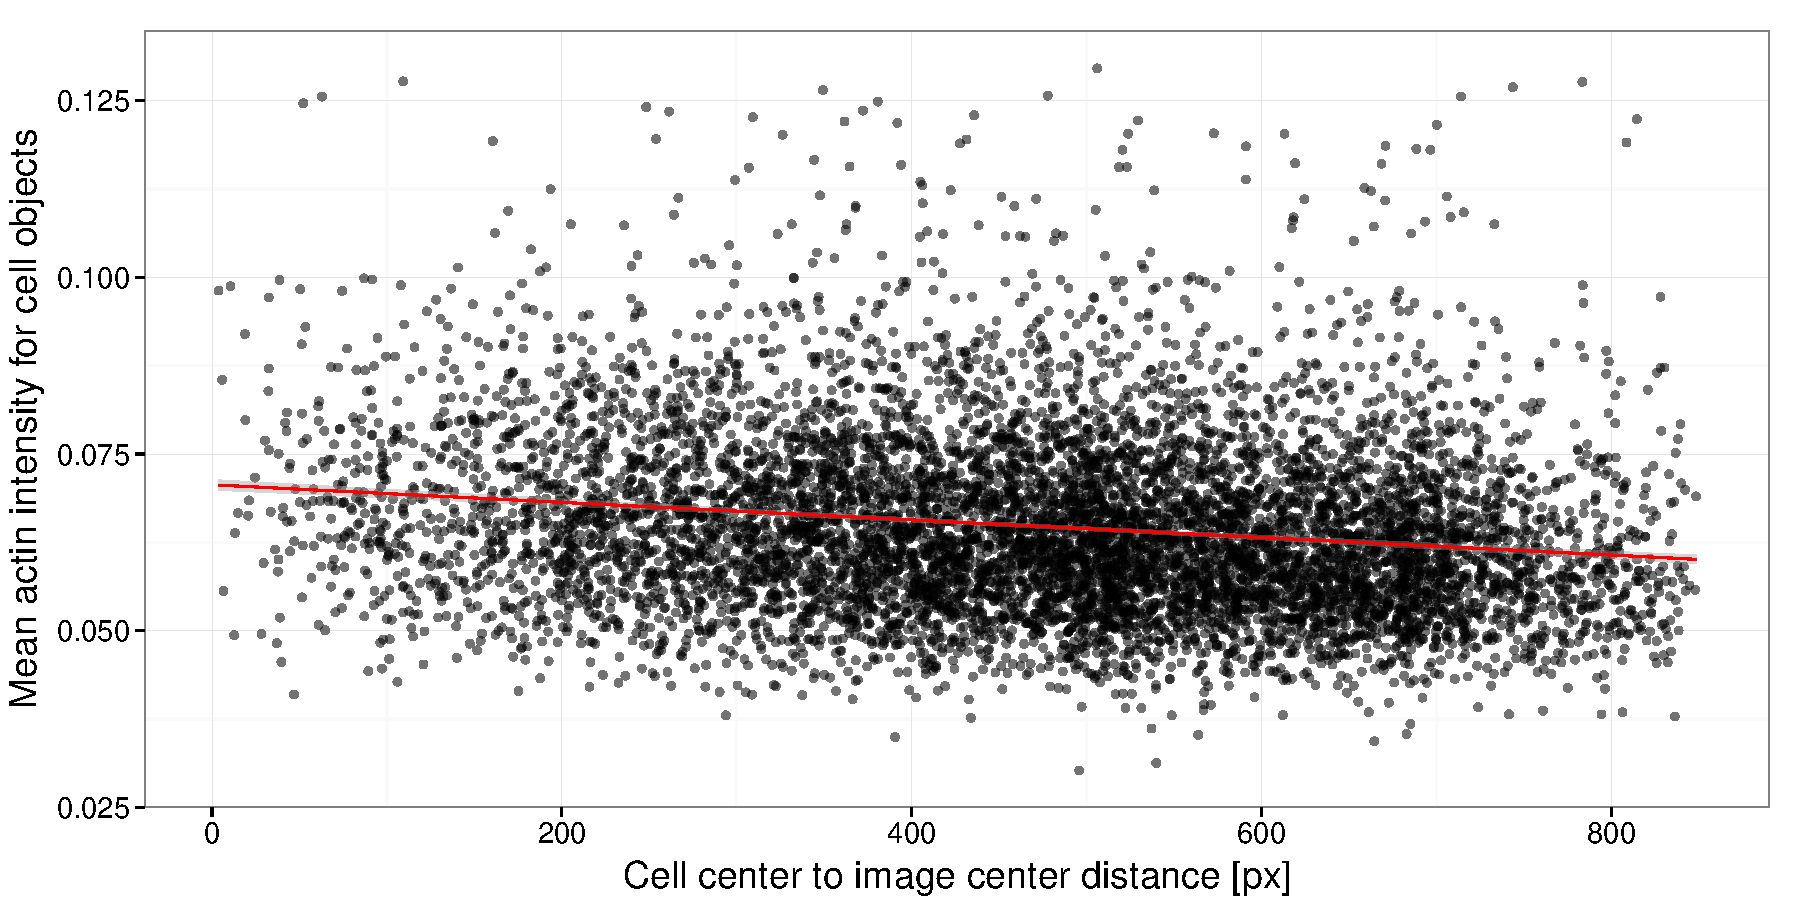
\includegraphics[width=.95\linewidth]{figures/R/location-trends-data-location-trend-1} 

}

\caption[Scatterplot visualization showing mean actin intensity against object distance from image center alongside a trend line.]{In order to illustrate the relationship between object location and feature values, a thinned out scatterplot (only a randomly sampled 1\% of datapoints are shown) of mean actin intensity against distance from image center is reproduced alongside a trend-line as calculated by gam of the \acrshort{cran} mgcv package. An approximately linear trend is discernible which can be found in many feature types.}\label{fig:data-location-trend}
\end{figure}


\end{knitrout}
